\documentclass{article}
\usepackage[utf8]{inputenc}
\usepackage{natbib}
\usepackage{graphicx}

\title{IF681 - Interface Usuário-Máquina}
\author{Bento Da Silva }
\date{November 2019}

\begin{document}
\maketitle
\section{Introdução}
    A disciplina Interface Usuário-Máquina é ministrada pelo Professor Alex Sandro Gomes no 4ª periodo do curso de Ciência da Computação no Centro de Informática da Universidade Federal de Pernambuco, CIN-UFPE. 
    Essa dicipina busca apresentar conceitors básicos de Design de interação homem-máquina, centrados no usuário, e Design Thinking para a concepção de sistema computacionais interativos.\cite{interface123disciplina}  

\begin{figure}[h!]
\centering
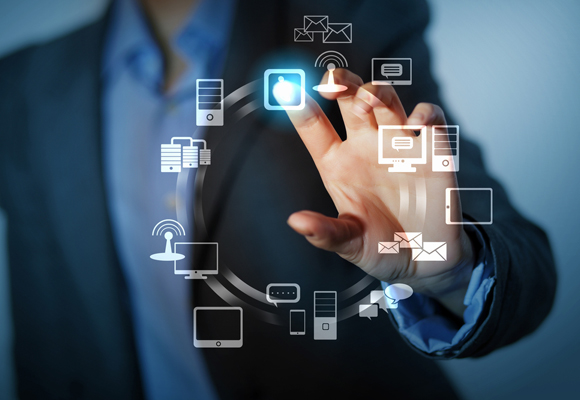
\includegraphics[scale=1.7]{interface-do-usuario.jpg}
\caption{Interface Usuário-Máquina}
\cite{interface123}
\label{fig:interface-do-usuario}
\end{figure}


\section{Relevância}
Na conclusão da diciplina é apresentado um picth, em que os estudantes precisam apresentar de forma clara e objetiva o projeto desenvolvido com a metodologia apresentada na diciplina. Essa apresentação demostra e ensina uma pratica essencial no mercado, estimulando os estudantes a defenderem e concluírem seus projetos, voltando suas soluções para a sociedade.  

\begin{figure}[h!]
\centering
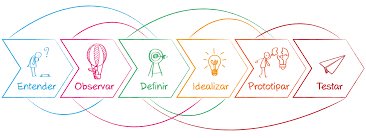
\includegraphics[scale=0.9]{designThinking.png}
\caption{Design Thinking}
\cite{interface1234353Thinking}
\label{fig:designThinking}
\end{figure}

\section{Relação com outras diciplinas}
A disciplina Interface Usuário-Máquina apresenta alta relação com o design e introduz conceitos primordiais para que os alunos possam trabalhar de forma multidiciplinar.


\begin{figure}[h!]
\centering
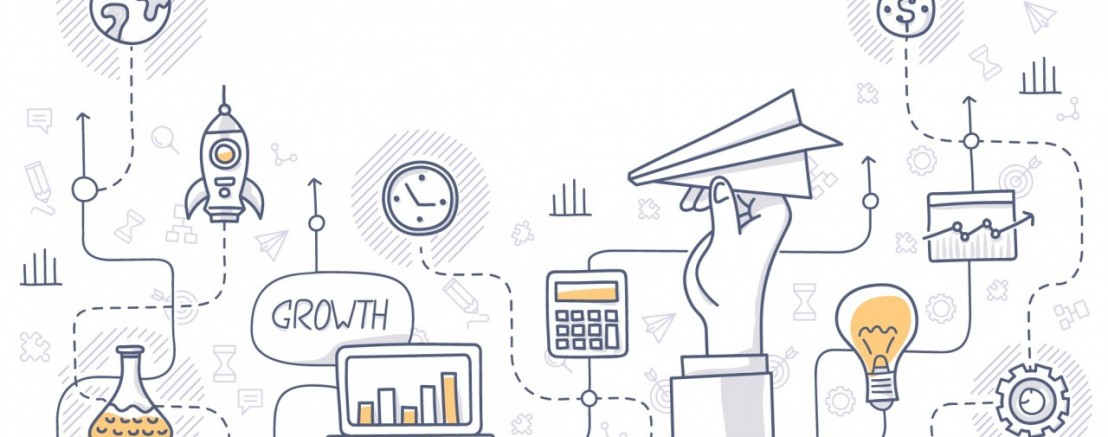
\includegraphics[scale=0.2]{design.jpg}
\caption{Interação com Design}
\cite{design}
\label{fig:design}
\end{figure}

\bibliographystyle{plain}
\bibliography{references}
\end{document}
